\chapter{My implementation, Julia + JuMP}
\label{ch:implementation}

I chose Julia with JuMP as the modelling environment. The toolchain had to be free and open source, fast and ergonomic. Julia targets the gap between C++ performance and Python ergonomics, and its community packages provide ready-to-use numerical tools. I also had prior experience in Python and wanted to learn Julia. My implementation is available on github \url{https://github.com/ceserik/SLapSim.jl}.

JuMP~\cite{Lubin2023} lets the user declare decision variables and constraints symbolically and uses automatic differentiation to supply first- and second-order derivatives to the solver. Through JuMP I use two NLP solvers: IPOPT~\cite{wachter_implementation_2006} for the CPU path and MadNLP~\cite{shin2021graph,shin2024accelerating} for both CPU and GPU paths. The full optimisation stack is shown in Figure~\ref{fig:opt_stack}.

The package InfiniteOpt.jl already implements several collocation schemes, but I chose to implement transcription myself. First, doing so gave a deeper understanding of the underlying methods. Second, InfiniteOpt abstracts away the low-level JuMP access, which may make custom mesh refinement, parametric vehicle models, and sensitivity analysis more difficult.

%\section{My optimization stack}

\begin{figure}[H]
	\centering
	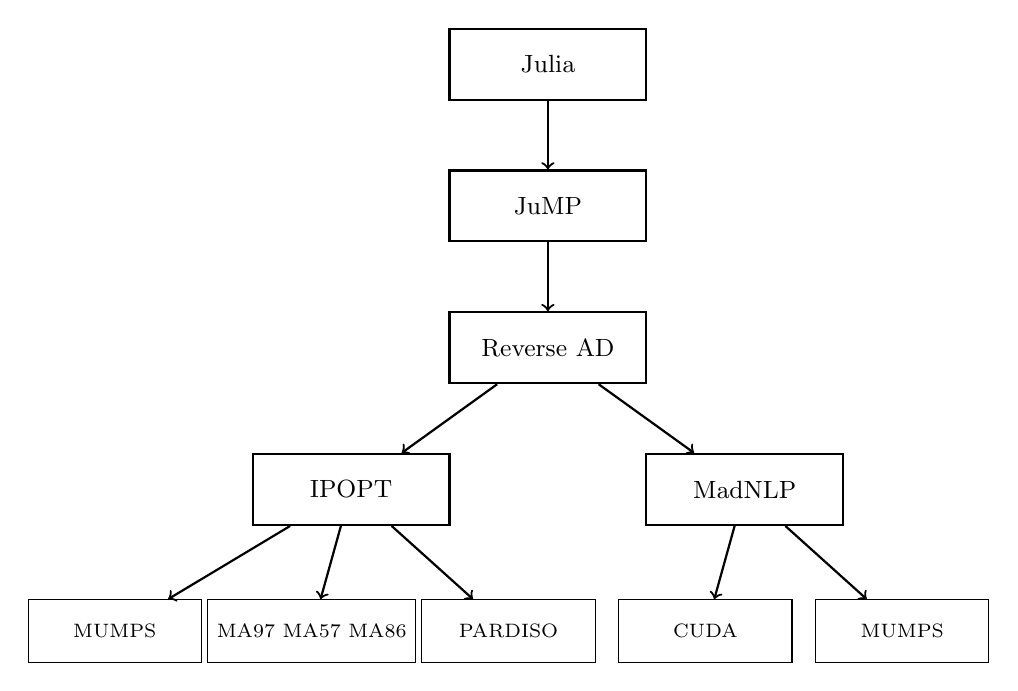
\begin{tikzpicture}[
			box/.style={rectangle, draw, thick, minimum width=2.5cm, minimum height=0.9cm, align=center, font=\small},
			leafbox/.style={rectangle, draw, minimum width=2.2cm, minimum height=0.8cm, align=center, font=\scriptsize},
			arr/.style={->, thick},
		]

		% Stack
		\node[box] (julia)  at (0, 0)   {Julia};
		\node[box] (jump)   at (0, -1.8) {JuMP};
		\node[box] (rad)    at (0, -3.6) {Reverse AD};
		\node[box] (ipopt)  at (-2.5, -5.4) {IPOPT};
		\node[box] (madnlp) at (2.5, -5.4)  {MadNLP};

		% IPOPT linear solvers
		\node[leafbox] (mumps)   at (-5.5, -7.2) {MUMPS};
		\node[leafbox] (hsl)     at (-3.0, -7.2) {MA97 MA57 MA86};
		\node[leafbox] (pardiso) at (-0.5, -7.2) {PARDISO};

		% MadNLP backends
		\node[leafbox] (cuda)     at (2.0, -7.2) {CUDA};
		\node[leafbox] (madmumps) at (4.5, -7.2) {MUMPS};

		% Main chain
		\draw[arr] (julia)  -- (jump);
		\draw[arr] (jump)   -- (rad);
		\draw[arr] (rad)    -- (ipopt);
		\draw[arr] (rad)    -- (madnlp);

		% IPOPT branches
		\draw[arr] (ipopt)  -- (mumps);
		\draw[arr] (ipopt)  -- (hsl);
		\draw[arr] (ipopt)  -- (pardiso);

		% MadNLP branches
		\draw[arr] (madnlp) -- (cuda);
		\draw[arr] (madnlp) -- (madmumps);

	\end{tikzpicture}
	\caption{Optimization software stack}
	\label{fig:opt_stack}
\end{figure}

\section{sensitivity Analysis}
I have used DiffOpt.jl~\cite{besancon2023diffopt} for the sensitivity analysis. By adding vehicle
parameters such as, mass, lift coefficient, CoG position etc. into
optimization as decisions variables fixed to a value by constraints. This added them to the algebraic model. Then the solution of minimum laptime can be differentiated by these parameters. Result of sensitivity analysis are on figure \ref{fig:sensitivity}.

\begin{figure}[H]
	\centering
	\makebox[\textwidth][c]{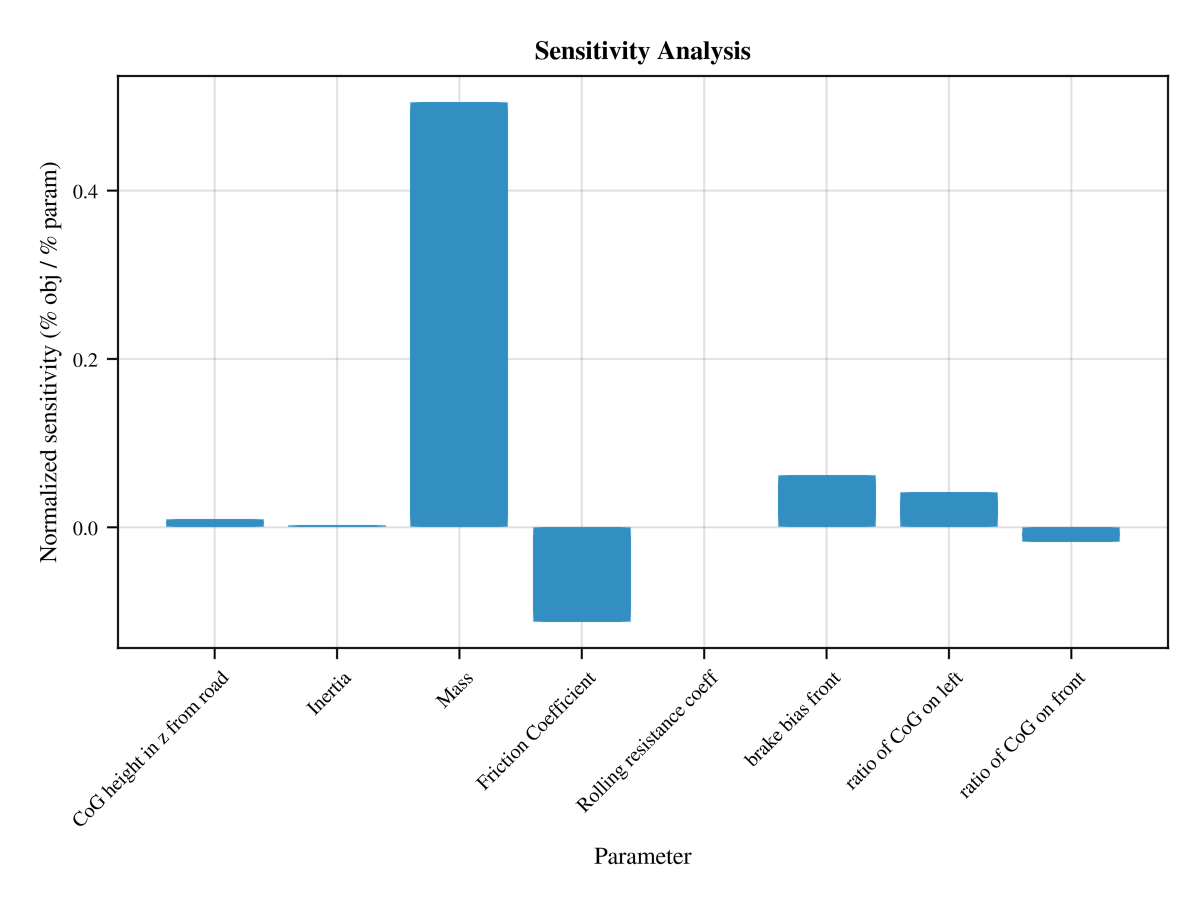
\includegraphics[width=1\textwidth]{../sync/sensitivity.png}}
	\caption{Node-interval ODE error for power-test case.}
	\label{fig:sensitivity}
\end{figure}

\section{Implemented nonlinear programming solvers}
Julia with JuMP offer high level interface which allows switching NLP solvers on single line. I have used Ipopt, MadNLP and Uno solver with preset filtersqp. Unfortunately the Uno solver was getting stuck, therefore it is not cosidered in this thesis.

Ipopt has built in Hessian aproximation strategy, in benchmark it proved to be inferior to automatic differentiation. Figure \ref{fig:nlp_flowchart_chosen} shows which solving methods were implemented and tested.
\begin{figure}[H]
\centering
\begin{tikzpicture}[
  >={Latex[length=2mm]},
  node distance=0.6cm and 0.15cm,
  every node/.style={font=\small, align=center},
  box/.style={draw, minimum height=0.7cm, inner sep=3pt},
  problem/.style={box},
  branch/.style={box, font=\small, text width=2.2cm},
  stagebox/.style={box, text width=2.6cm, font=\footnotesize},
  deriv/.style={box, text width=1.4cm, font=\footnotesize},
  terminal/.style={box, line width=1pt},
  chosen/.style={fill=green!30}
]

\node[problem] (nlp) {Transcribed nonlinear programming problem};

\node[branch, below=0.75cm of nlp, xshift=-1.5cm] (sqp) {Sequential\\Quadratic\\Programming};
\node[branch, below=0.75cm of nlp, xshift=1.5cm, chosen] (ipm) {Interior\\Point\\Methods};

\node[problem, below=3cm of nlp] (need) {Compute derivatives};

\node[deriv, below=1cm of need] (fd) {Finite\\differences};
\node[deriv, left=of fd]  (sym)  {Symbolic};
\node[deriv, left=of sym] (anal) {Analytic};
\node[deriv, right=of fd, chosen] (ad)   {Automatic\\diff.};
\node[deriv, right=of ad, chosen] (qn)   {Quasi-\\Newton\\methods};

\node[terminal, below=3cm of need] (newton) {Assemble linear system\\\textbf{Newton step}};

\draw[->] (nlp) -- (sqp);
\draw[->, very thick, green!60!black] (nlp) -- (ipm);
\draw[->] (sqp) -- (need);
\draw[->, very thick, green!60!black] (ipm) -- (need);

\draw[->] (need) -- (anal);
\draw[->] (need) -- (sym);
\draw[->] (need) -- (fd);
\draw[->, very thick, green!60!black] (need) -- (ad);
\draw[->, very thick, green!60!black] (need) -- (qn);

\draw[->] (anal) -- (newton);
\draw[->] (sym)  -- (newton);
\draw[->] (fd)   -- (newton);
\draw[->, very thick, green!60!black] (ad)   -- (newton);
\draw[->, very thick, green!60!black] (qn)   -- (newton);

\end{tikzpicture}
\caption{NLP solution flow with the methods used in this thesis highlighted in green}
\label{fig:nlp_flowchart_chosen}
\end{figure}
\section{Implementation of mesh refinement}
I have implemented p and h method for mesh refinement. Error calculation is implemented using comparing the result of interpolated value at the and of segment and the result of simulation using Rodas4() solver.

To calculate the error at the end of each segment, the interpolated controls and intial states are plugged into Rodas4 IVP solver. Then this result is compared to the states from transcription method. If error between states in absolute vlaue is larger than user defined threshold, the segment is halved. This one of the simpler estimators of discretization error.


Figure \ref{fig:power_node_controls} shows that
error along track is not distributed equaly. Error is localised around areas
with large jump in controls. These areas need finer sampling. P methods cannot
focus these specific points directly, they focus entire trajectory.

The errors are concentrated around the discontinuity of controls, where the
behaviour of the vehicle is more complex/ requiring high order or finer
approximation see Figure \ref{fig:power_node_controls}. Time optimal control of car around track has many discontinuities and therefore p methods are not a good fit for this use.


\begin{figure}[H]
    \centering
    \makebox[\textwidth][c]{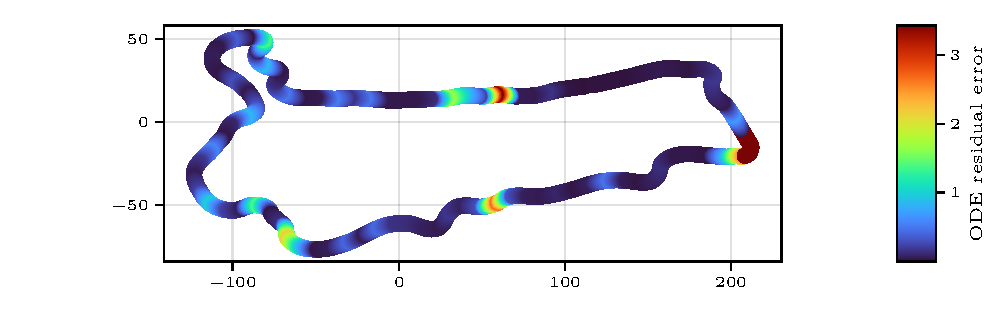
\includegraphics[width=1\textwidth]{../sync/thesisImages/mesh_refinement_fscz_error_iter0.pdf}}
    \caption{Node-interval ODE error for power-test case.}
    \label{fig:power_node_controls}
\end{figure}

\begin{figure}[H]
    \centering
    \makebox[\textwidth][c]{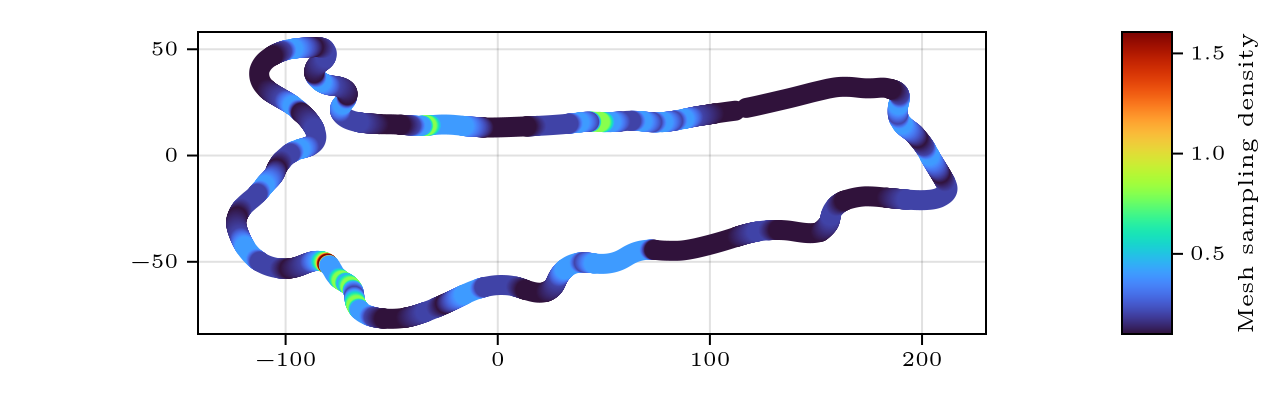
\includegraphics[width=1\textwidth]{../sync/thesisImages/mesh_refinement_fscz_density_iter10.png}}
    \caption{Node-interval ODE error for power-test case.}
    \label{fig:power_node_controls}
\end{figure}



\begin{figure}[H]
    \centering
    \makebox[\textwidth][c]{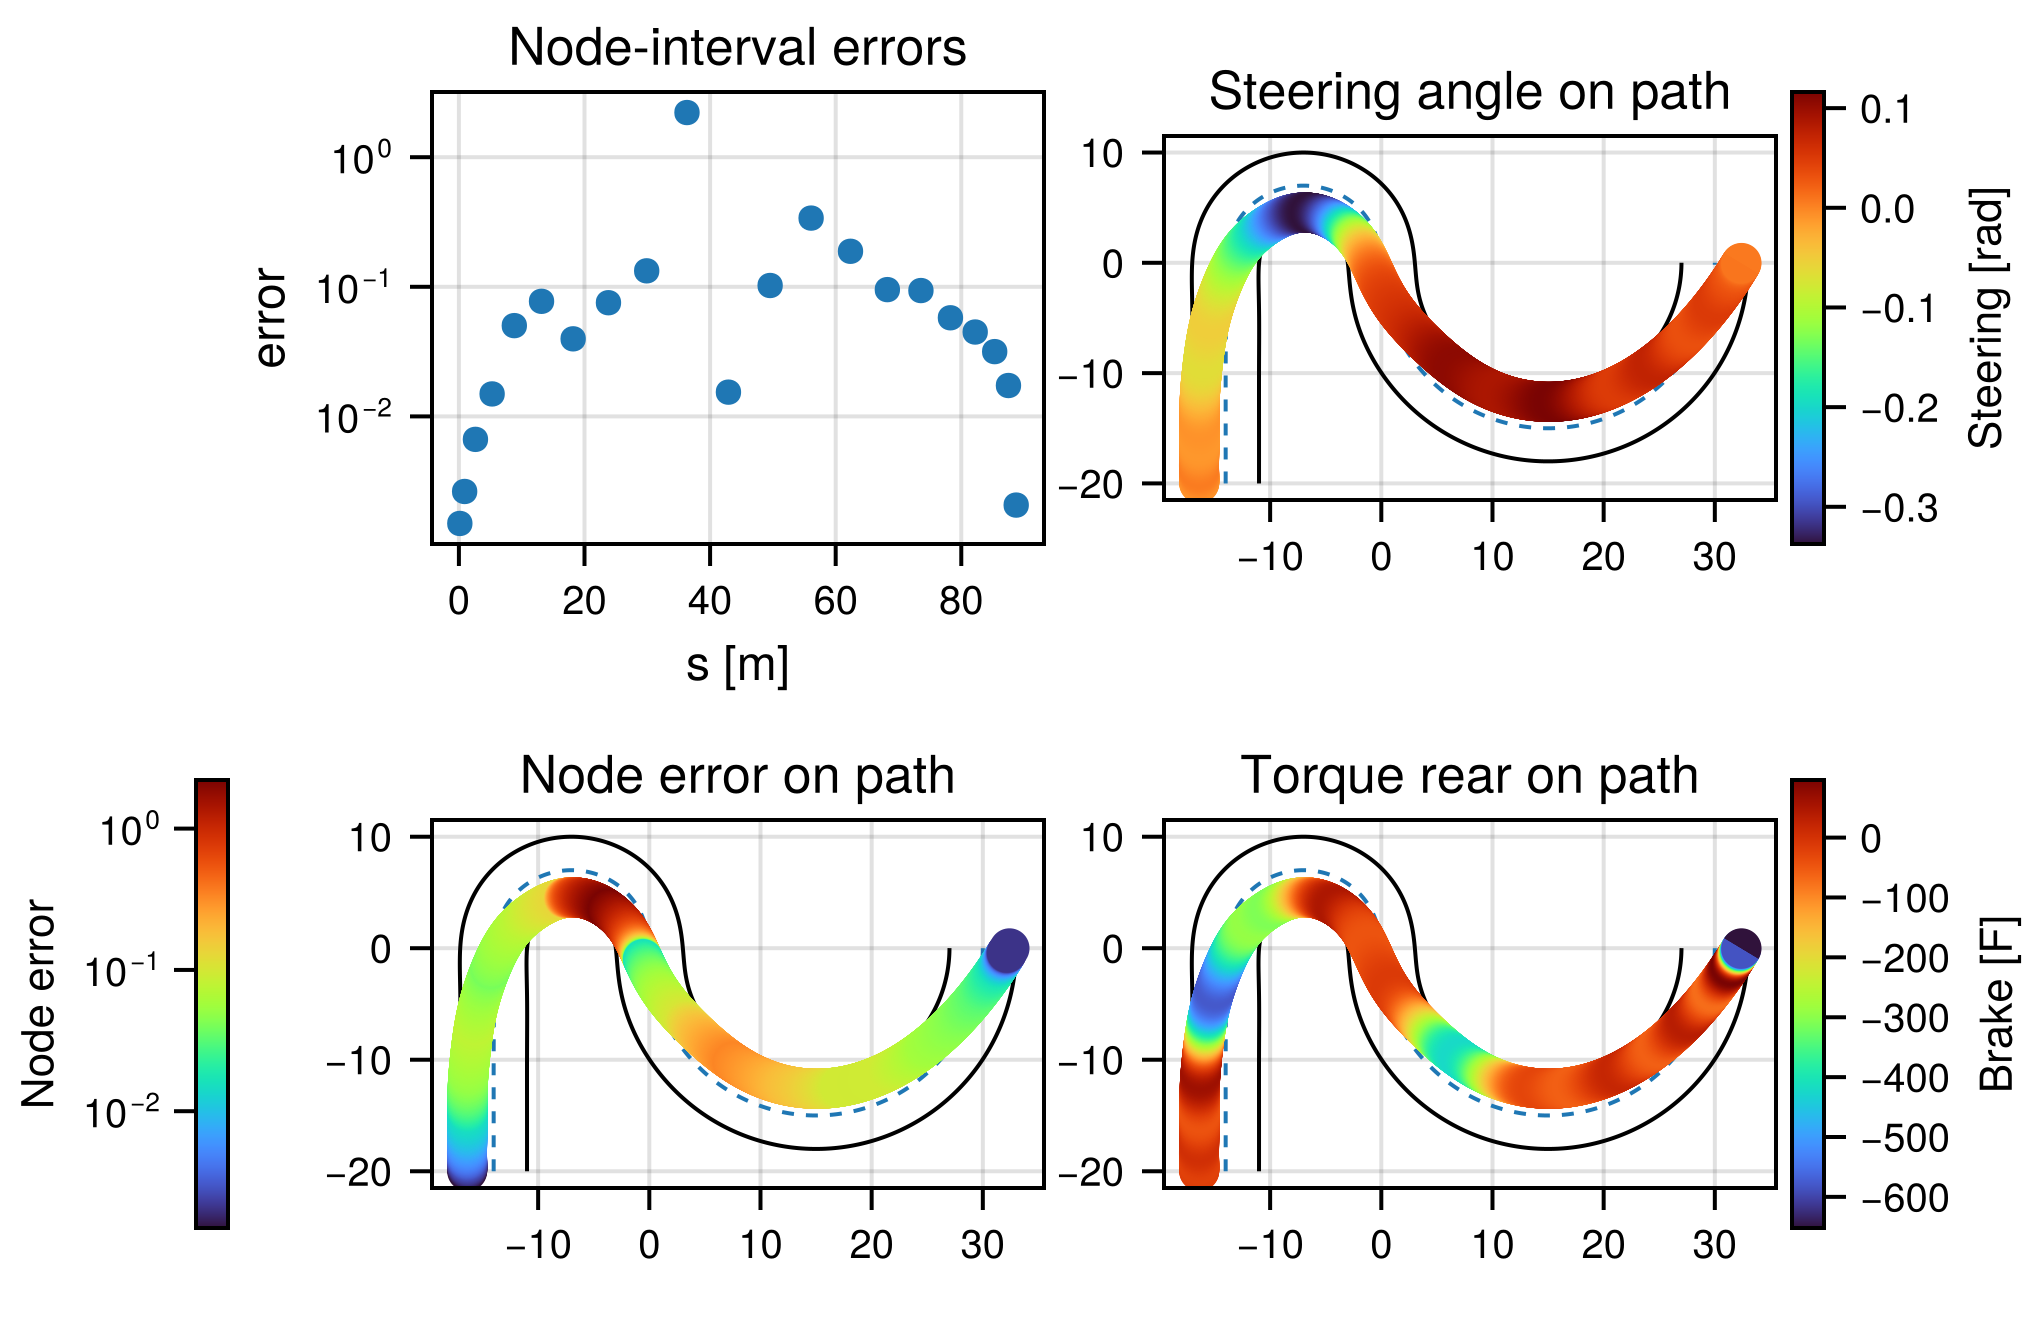
\includegraphics[width=1\textwidth]{../sync/p_methodplots/power_summary2x2.png}}
    \caption{Node-interval ODE error for power-test case.}
    \label{fig:power_node_controls}
\end{figure}



\begin{figure}[H]
\centering
\begin{tikzpicture}[
  >={Latex[length=2mm]},
  node distance=0.7cm and 0.35cm,
  method/.style={draw, text width=2.4cm, minimum height=0.9cm, align=center, font=\small, inner sep=3pt},
  layer/.style={draw, minimum height=0.8cm, inner sep=4pt, align=center, font=\normalsize\bfseries},
  chosen/.style={fill=green!30}
]

\node[method, chosen]      (p)   {$p$-refinement\\(raise polynomial degree)};
\node[method, chosen, right=of p]  (h)   {$h$-refinement\\(subdivide segments)};
\node[method, right=of h]  (hp)  {$hp$-refinement\\(p first, then h)};
\node[method, right=of hp] (ph)  {$ph$-refinement\\(h first, then p)};

\node[layer, above=1cm of $(p.north)!0.5!(ph.north)$] (mesh)
  {Mesh refinement strategy};

\draw[->, very thick, green!60!black] (mesh.south) -- (p.north);
\draw[->, very thick, green!60!black] (mesh.south) -- (h.north);
\draw[->] (mesh.south) -- (hp.north);
\draw[->] (mesh.south) -- (ph.north);

\end{tikzpicture}
\caption{Mesh refinement layer with the strategies implemented in this thesis highlighted in green}
\label{fig:mesh_refinement_chosen}
\end{figure}

\section{Implementation of collocation methods}
\begin{figure}[H]
\centering
\begin{tikzpicture}[
  >={Latex[length=2mm]},
  node distance=0.55cm and 0.18cm,
  basis/.style={draw, text width=1.4cm, minimum height=0.8cm, align=center, font=\scriptsize, inner sep=2pt},
  scheme/.style={draw, text width=3.2cm, minimum height=0.8cm, align=center, font=\small, inner sep=3pt},
  form/.style={draw, text width=1.25cm, minimum height=0.6cm, align=center, font=\scriptsize, inner sep=2pt},
  layer/.style={draw, minimum height=0.8cm, inner sep=4pt, align=center, font=\normalsize\bfseries},
  chosen/.style={fill=green!30}
]

\node[basis]                    (cheb) {Chebyshev\\I \& II};
\node[basis, right=of cheb]     (her)  {Hermite};
\node[basis, right=of her]      (lag)  {Laguerre};
\node[basis, right=of lag, chosen] (leg)  {Legendre};
\node[basis, right=of leg]      (alag) {Assoc.\\Laguerre};
\node[basis, right=of alag]     (geg)  {Gegenbauer};
\node[basis, right=of geg]      (jac)  {Jacobi};

\node[layer, above=1cm of $(cheb.north)!0.5!(jac.north)$] (trans)
  {Transcription:\\orthogonal polynomial basis};

\foreach \n in {cheb,her,lag,alag,geg,jac}
  \draw[->] (trans.south) -- (\n.north);
\draw[->, very thick, green!60!black] (trans.south) -- (leg.north);

\node[scheme, chosen, below=1.8cm of leg] (lgr) {Legendre--Gauss--Radau\\(LGR) Quadrature};
\node[scheme, chosen, left=of lgr]  (lg)  {Legendre--Gauss\\(LG) Quadrature};
\node[scheme, chosen, right=of lgr] (lgl) {Legendre--Gauss--Lobatto\\(LGL) Quadrature};

\draw[->, very thick, green!60!black] (leg.south) -- (lg.north);
\draw[->, very thick, green!60!black] (leg.south) -- (lgr.north);
\draw[->, very thick, green!60!black] (leg.south) -- (lgl.north);

\foreach \n in {cheb,her,lag,alag,geg,jac}
  \node[font=\Large, below=0.35cm of \n] {$\vdots$};

\node[form, below=0.8cm of lg, xshift=-0.85cm]         (lg-int)  {Integral};
\node[form, chosen, below=0.8cm of lg, xshift=0.85cm]  (lg-diff) {Differ.};
\draw[->] (lg.south) -- (lg-int.north);
\draw[->, very thick, green!60!black] (lg.south) -- (lg-diff.north);

\node[form, below=0.8cm of lgr, xshift=-0.85cm]         (lgr-int)  {Integral};
\node[form, chosen, below=0.8cm of lgr, xshift=0.85cm]  (lgr-diff) {Differ.};
\draw[->] (lgr.south) -- (lgr-int.north);
\draw[->, very thick, green!60!black] (lgr.south) -- (lgr-diff.north);

\node[form, chosen, below=0.8cm of lgl, xshift=-0.85cm] (lgl-int)  {Integral};
\node[form, below=0.8cm of lgl, xshift=0.85cm]          (lgl-diff) {Differ.};
\draw[->, very thick, green!60!black] (lgl.south) -- (lgl-int.north);
\draw[->] (lgl.south) -- (lgl-diff.north);

\end{tikzpicture}
\caption{Transcription layer with the methods used in this thesis highlighted in green}
\label{fig:transcription_chosen}
\end{figure}


\section{My collocation}
my mesh refinbment error calc + my methods implemented

\section{my mesh refinment}
ode error

\section{My car models}
PUT CAR MODELS HERE
\subsection{singletrack}
\subsection{Formula Student twintrack}
\subsection{FormulaE}
\subsection{Bus}
%\subsection{my tires}

%\subsection{my suspensions}

\section{Benchmark tracks}
The following tracks are used in the benchmark in
Section~\ref{sec:benchmark}. They cover real Formula Student layouts
(FSCZ, FSG), a Formula~E street circuit (Berlin) and two synthetic
geometries (DoubleTurn, FigureEight).

\begin{figure}[H]
    \centering
    \begin{subfigure}[t]{0.48\textwidth}
        \centering
        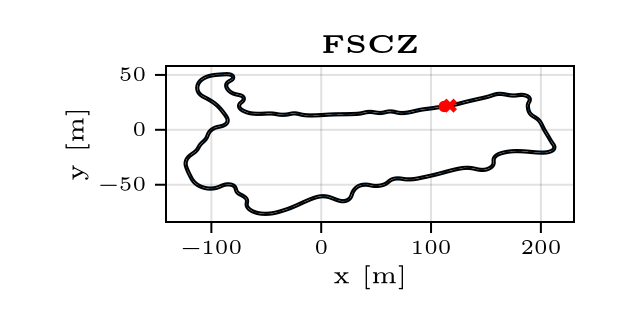
\includegraphics[width=\linewidth]{../sync/thesisImages/benchmark_track_FSCZ.png}
        \caption{Formula Student Czech track}
        \label{fig:track_fscz}
    \end{subfigure}\hfill
    \begin{subfigure}[t]{0.48\textwidth}
        \centering
        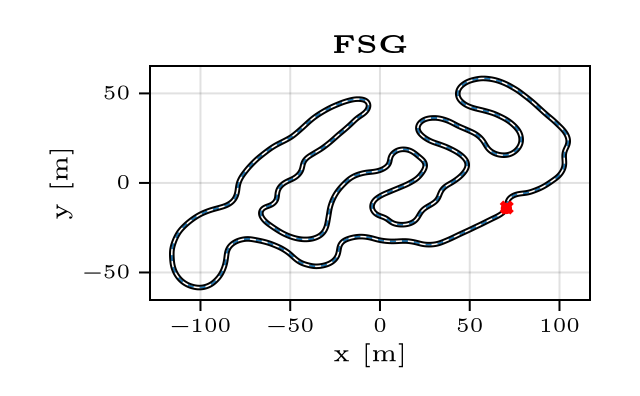
\includegraphics[width=\linewidth]{../sync/thesisImages/benchmark_track_FSG.png}
        \caption{Formula Student Germany track}
        \label{fig:track_fsg}
    \end{subfigure}

    \vspace{0.5em}
    \begin{subfigure}[t]{0.48\textwidth}
        \centering
        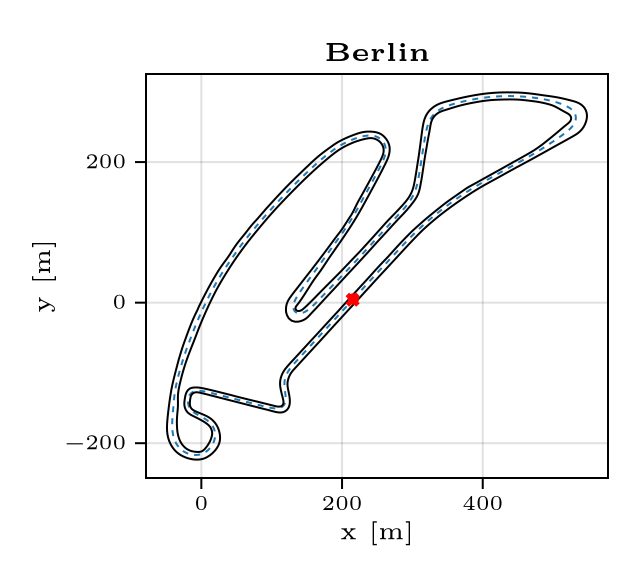
\includegraphics[width=\linewidth]{../sync/thesisImages/benchmark_track_Berlin.png}
        \caption{Berlin (Formula~E)}
        \label{fig:track_berlin}
    \end{subfigure}\hfill
    \begin{subfigure}[t]{0.48\textwidth}
        \centering
        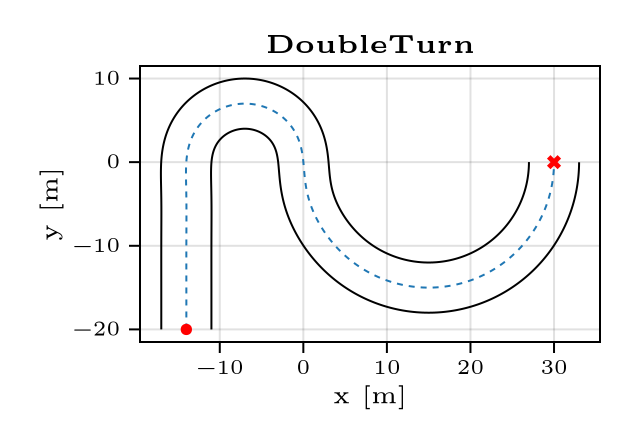
\includegraphics[width=\linewidth]{../sync/thesisImages/benchmark_track_DoubleTurn.png}
        \caption{DoubleTurn}
        \label{fig:track_doubleturn}
    \end{subfigure}

    \vspace{0.5em}
    \begin{subfigure}[t]{0.48\textwidth}
        \centering
        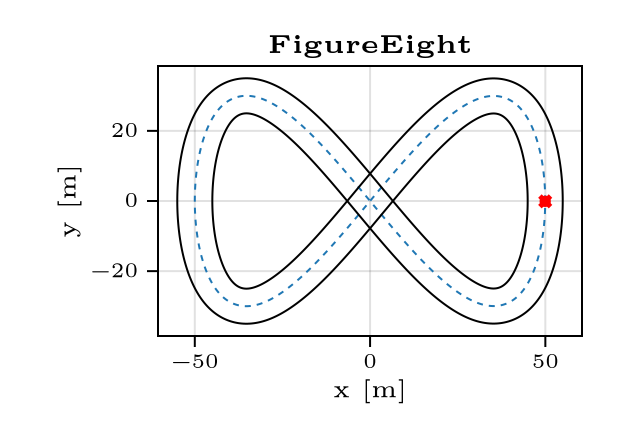
\includegraphics[width=\linewidth]{../sync/thesisImages/benchmark_track_FigureEight.png}
        \caption{FigureEight}
        \label{fig:track_figureeight}
    \end{subfigure}
    \caption{Tracks used in the solver/transcription benchmark.}
    \label{fig:benchmark_tracks}
\end{figure}

\section{Actual constriants, exampleconstraints like cannot leave road}